\documentclass[10pt,letterpaper]{article}

\usepackage{amsmath}
\usepackage{amssymb}
\usepackage{array}
\usepackage[greek,english]{babel}
\usepackage[aboveskip=1pt,labelfont=bf,labelsep=period,justification=raggedright,singlelinecheck=off]{caption}
   \renewcommand{\figurename}{Fig}
\usepackage{changepage}
\usepackage{cite}
\usepackage{dcolumn}
   \newcolumntype{d}[1]{D{.}{.}{#1}}
\usepackage{epstopdf}
\usepackage{fancyhdr}
\usepackage{float}
\usepackage[top=0.85in,left=2.75in,footskip=0.75in]{geometry}
\usepackage{graphicx}
\usepackage{hyperref}
\usepackage{lastpage}
\usepackage[right]{lineno}
\usepackage{marvosym}
\usepackage[nopatch=eqnum]{microtype}
   \DisableLigatures[f]{encoding=*,family=*}
\usepackage{nameref}
\usepackage{pdflscape}
\usepackage{soul}
\usepackage{subcaption}
\usepackage[table]{xcolor}
\usepackage{textcomp}

\newcolumntype{+}{!{\vrule width 2pt}}

\newlength\savedwidth
\newcommand\thickcline[1]{%
   \noalign{\global\savedwidth\arrayrulewidth\global\arrayrulewidth 2pt}%
   \cline{#1}%
   \noalign{\vskip\arrayrulewidth}%
   \noalign{\global\arrayrulewidth\savedwidth}%
}

\newcommand\thickhline{\noalign{\global\savedwidth\arrayrulewidth\global\arrayrulewidth 2pt}%
\hline
\noalign{\global\arrayrulewidth\savedwidth}}

\raggedright
\setlength{\parindent}{0.5cm}
\textwidth 5.25in
\textheight 8.75in

\bibliographystyle{plos2015}

\makeatletter
\renewcommand{\@biblabel}[1]{\quad#1.}
\makeatother

% \pagestyle{myheadings}
\pagestyle{fancy}
\fancyhf{}
% \setlength{\headheight}{27.023pt}
% \lhead{\includegraphics[width=2.0in]{PLOS-submission.eps}}
\rfoot{\thepage/\pageref{LastPage}}
\renewcommand{\headrulewidth}{0pt}
\renewcommand{\footrule}{\hrule height 2pt \vspace{2mm}}
\fancyheadoffset[L]{2.25in}
\fancyfootoffset[L]{2.25in}
\lfoot{\today}

\begin{document}


%%%%%%%%%%%%%%%%%%%%%%%%%%%%%
% EXEMPLARY TASK OF STUDY 2 %
%%%%%%%%%%%%%%%%%%%%%%%%%%%%%
\paragraph*{S5 Appendix}
{\bf Exemplary Task of Study 2}

\noindent $A$ and $B$ have cut $500$ logs each $[A$ has cut $200$ and $B$ has cut $800$ logs$]$.
So both persons have cut a total of $1,000$ logs.
In the empty spaces below, please make the distribution to both people that you think is most just.\vspace{4ex}

\begin{minipage}[t]{.4\linewidth}
   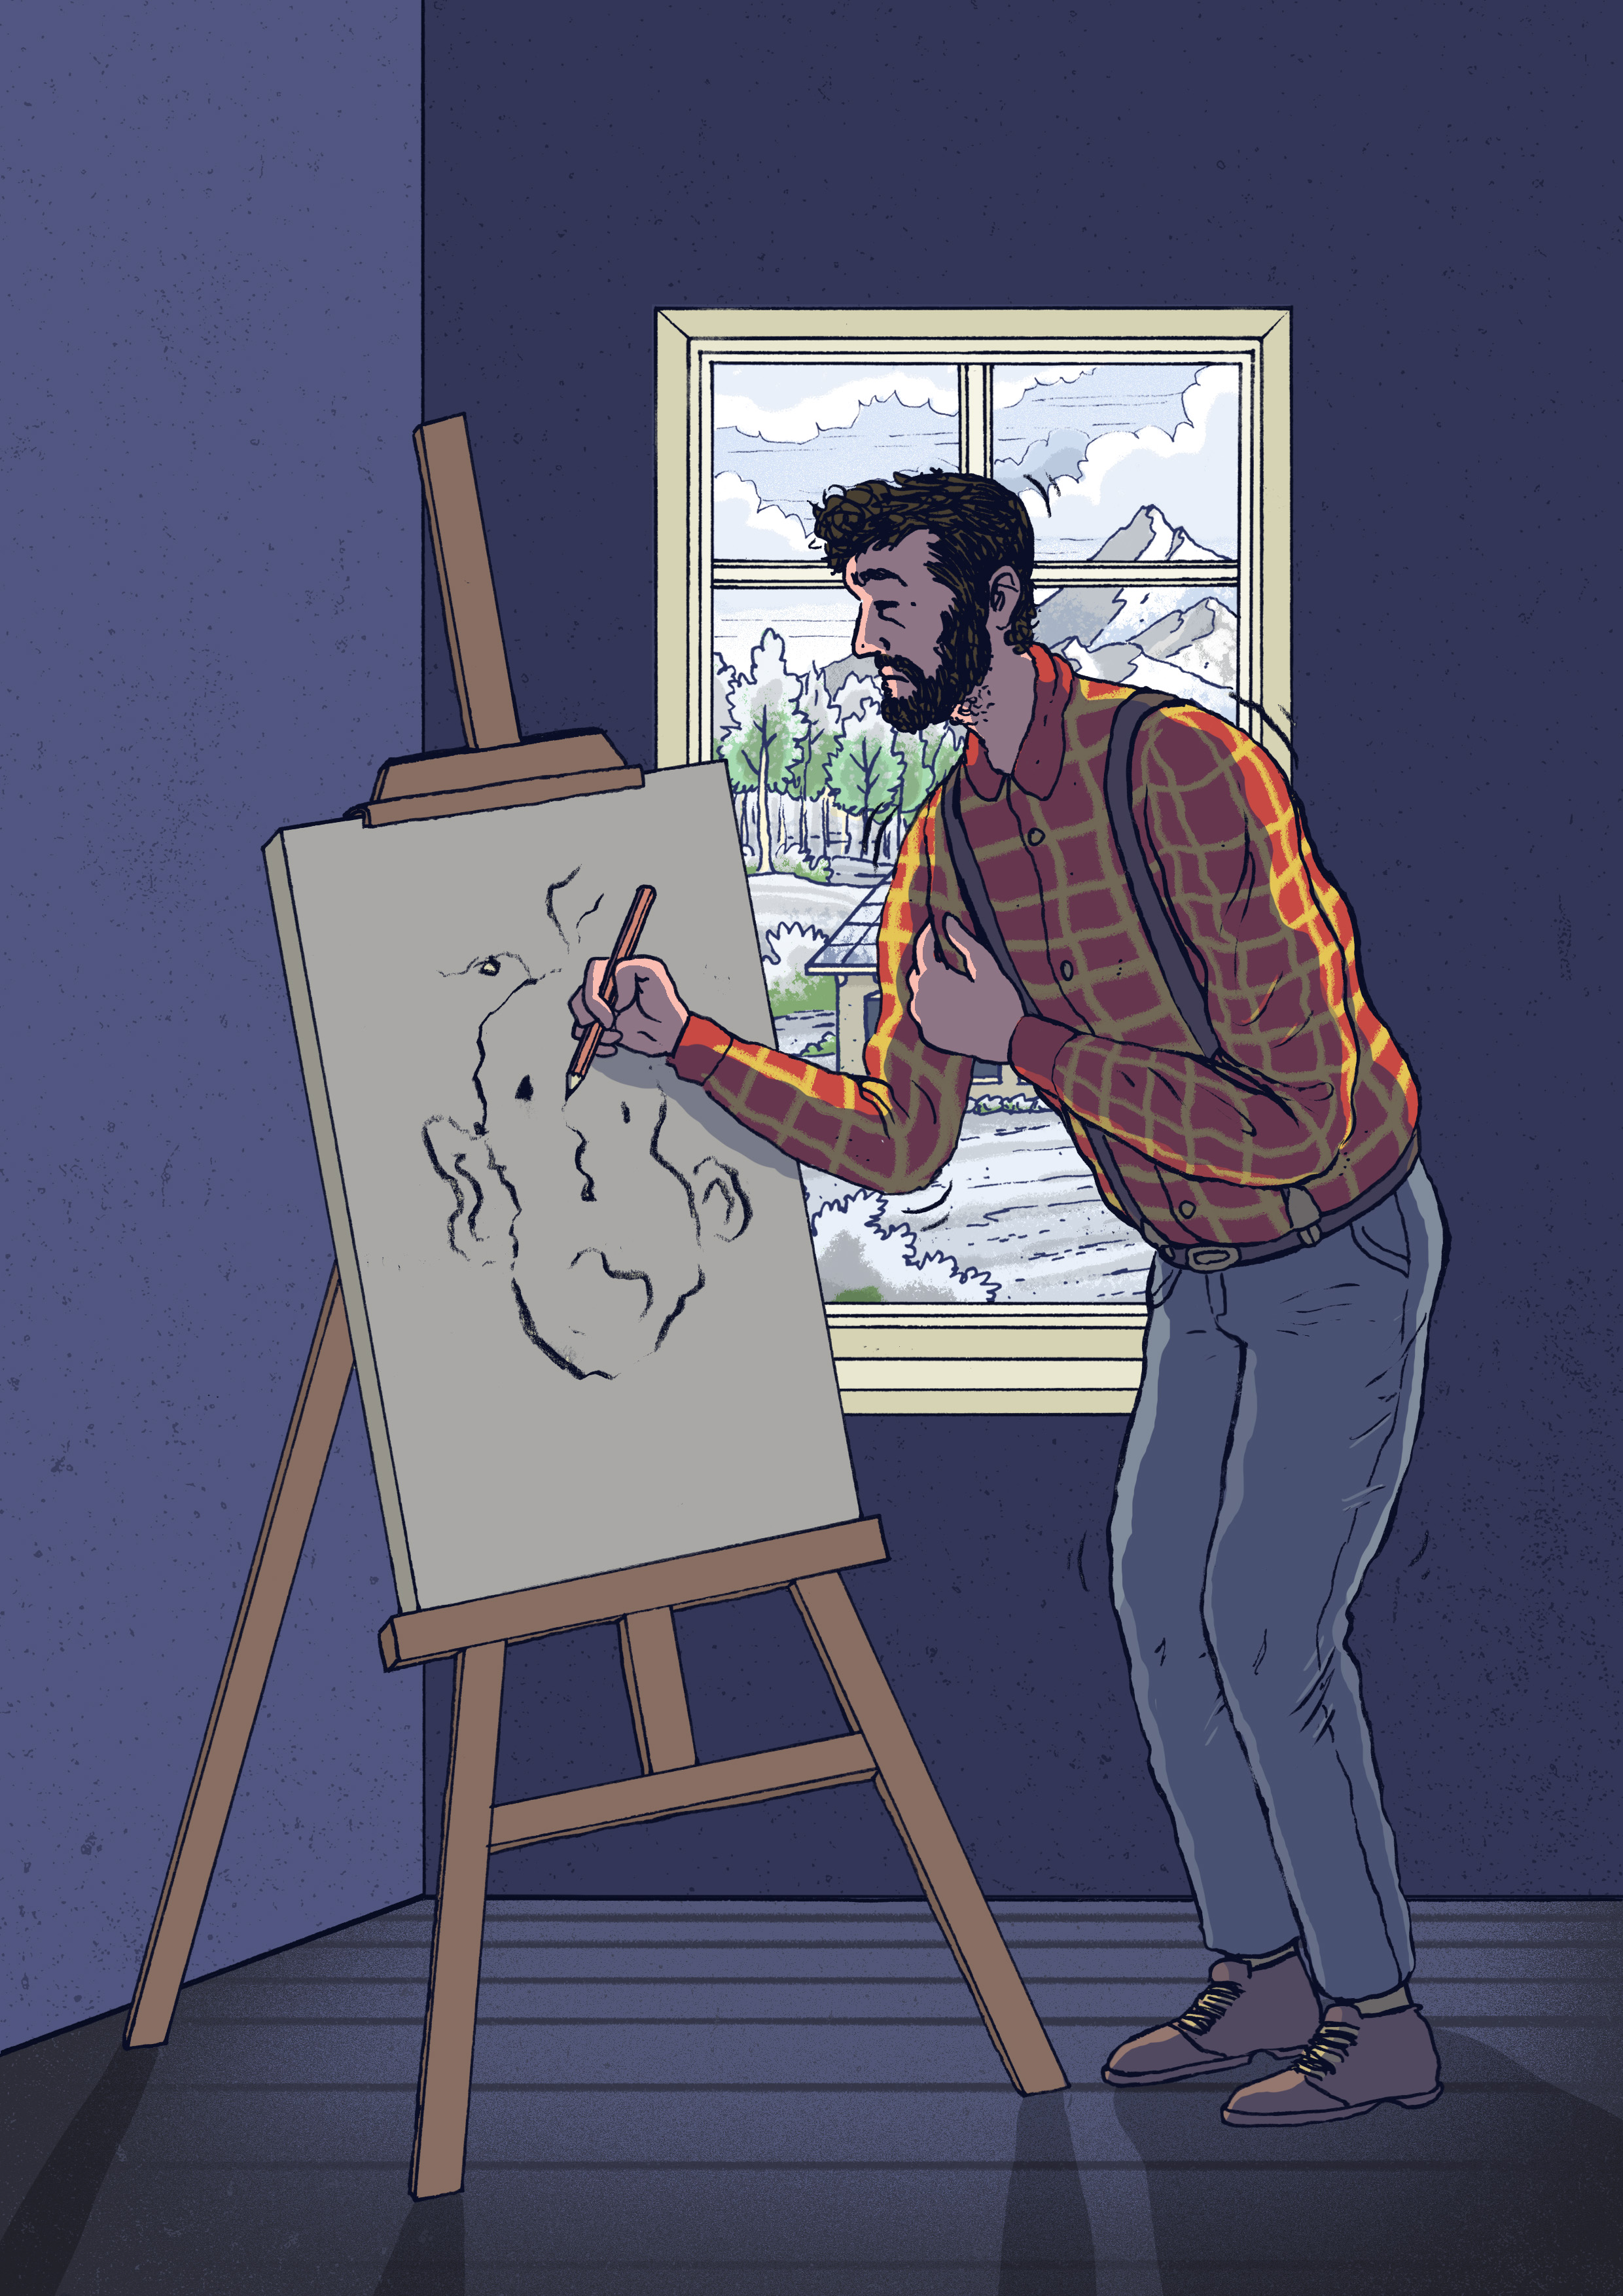
\includegraphics[width=\linewidth]{figures/figure_1_d.jpg}
   $A$ needs the wood so that their studio does not become unusable in the winter.\\[2ex] $A$ should receive \_\_\_ logs of wood.
\end{minipage}
\hfill
\begin{minipage}[t]{.4\linewidth}
   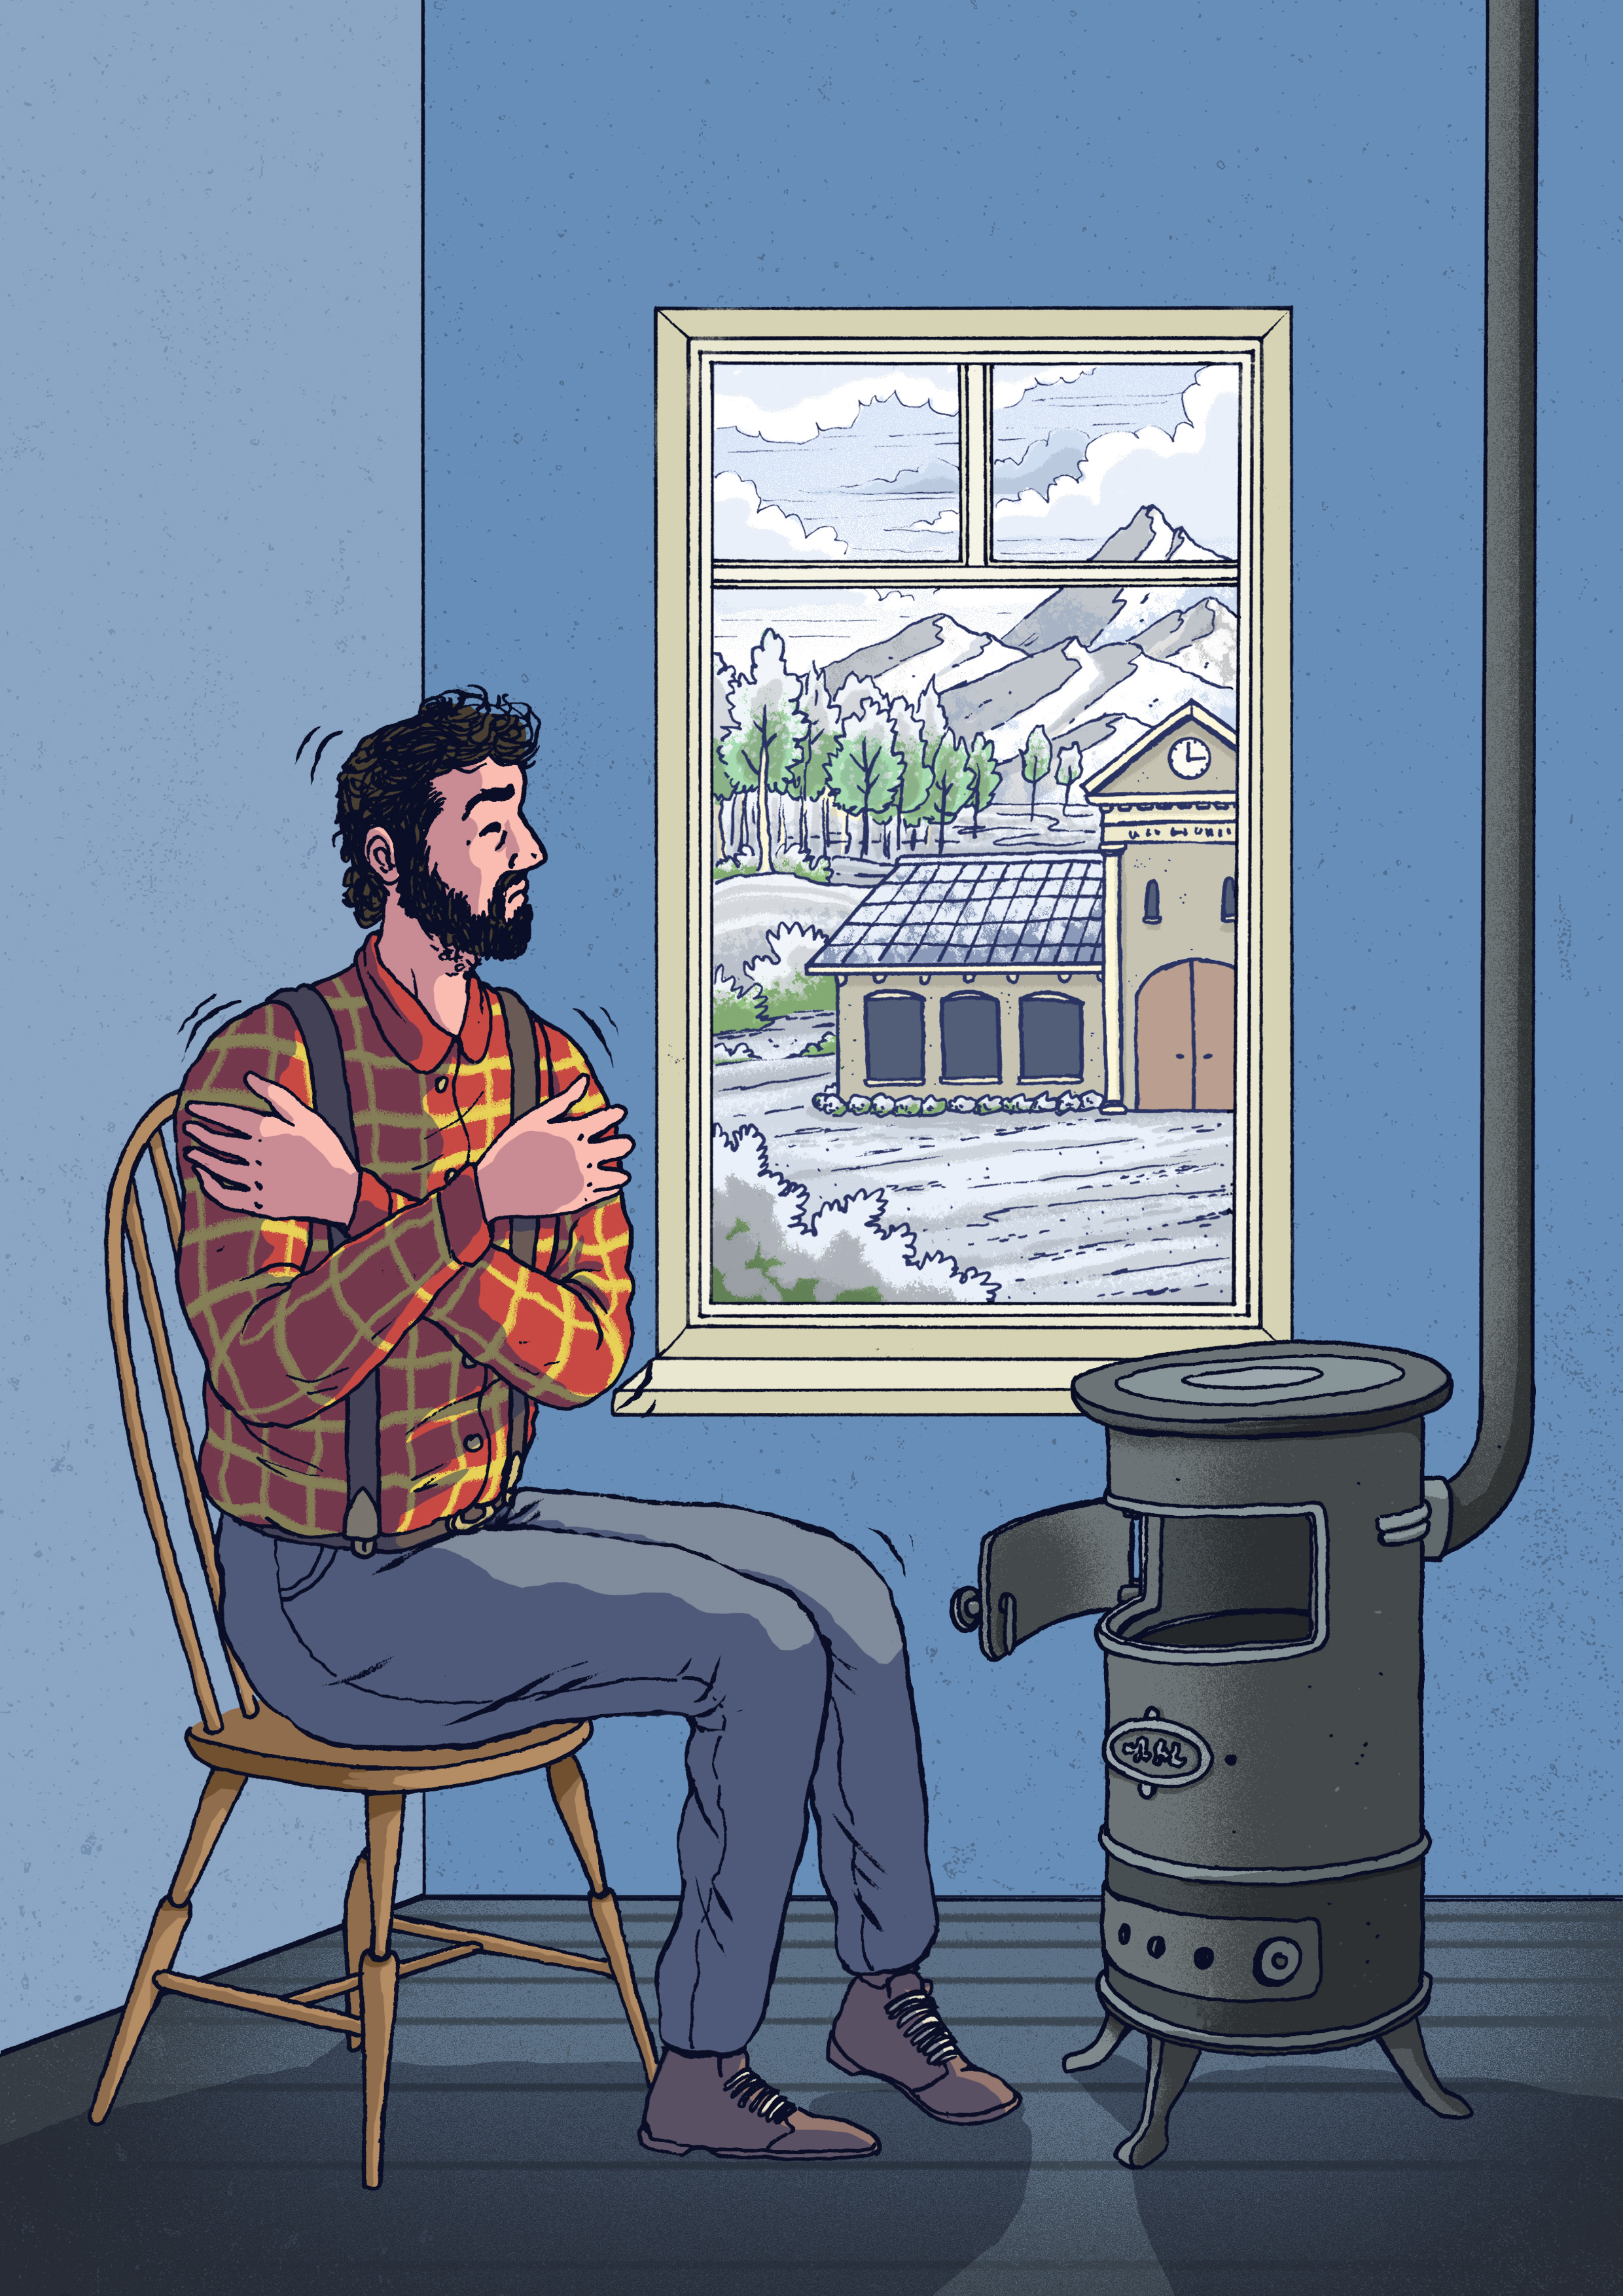
\includegraphics[width=\linewidth]{figures/figure_1_b.jpg}
   $B$ needs the wood to avoid freezing in the winter.\\[5ex] $B$ should receive \_\_\_ logs of wood.
\end{minipage}

\end{document}
